\documentclass[marginline,noindent,answers,adobefonts]{BHCexam}	
\renewcommand{\kongbai}{\vspace{15em}}

\newcommand{\xl}[2]{\vv{#1}\bm\cdot\vv{#2}}
\newcommand{\zj}[1]{\vspace{-1em}\begin{center}\begin{tikzpicture}#1\end{tikzpicture}\end{center}}
\newcommand{\yc}[1]{\vspace{-1em}\begin{flushright}\begin{tikzpicture}#1\end{tikzpicture}\end{flushright}}
%\coordinate[label=right:\footnotesize$E$](e) at(intersection of a--f and b--d);%intersection

\begin{document}
\begin{questions}
\qs 正方体$ ABCD-A_1B_1C_1D_1 $的棱长为1,点$ P,~Q,~R $分别是棱$ AA_1,~A_1B_1,~A_1D_1 $的中点,以$ \triangle PQR $为底面做正三棱柱,若此三棱柱另一底面三个顶点也都在该正方体表面上,则这个正三棱柱的高$ h= $\tk.
\vspace{-2em}
\begin{center}
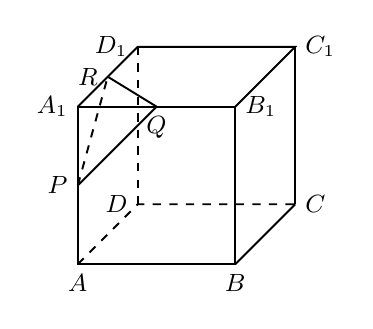
\begin{tikzpicture}[line width=0.7 pt,scale=1]
%\draw[help lines] (0,0) grid (3,3);
\draw (0,0) node[below](A) {\small$A$}--(2,0) node[below](B){\small$B$}--(2,2) node[right](B1){\small$B_1$}--(0,2) node[left](A1) {\small$A_1$}--(0,0)--cycle;
\draw[dashed] (0,0)--(0.76,0.76) node[left](D){\small$D$}--(2.76,0.76) node[right](C){\small$C$};
\draw (2.76,0.76)--(2,0);
\draw (0,2) --(0.76,2.76)node[left](D1){\small$D_1$}--(2.76,2.76)node[right](C1){\small$C_1$}--(2,2);
\draw [dashed](0.76,2.76)--(0.76,0.76) ;
\draw (2.76,2.76)--(2.76,0.76);
%\draw [dashed](0.76,2.76)--(2.38,0.38) node[right](E) {\small$E$};
\coordinate[label=left:\small$P$] (P) at (0,1);
\coordinate[label=left:\small$R$] (R) at (0.38,2.38);
\coordinate[label=below:\small$Q$] (Q) at (1,2);
\draw (P)--(Q)--(R) ;
\draw [dashed](P)--(R);
%\coordinate[label=left:$S$] (S) at ($(P)!0.5!(Q)$);
\end{tikzpicture}
\end{center}
\qs 如图,已知正方体$ABCD-A_1B_1C_1D_1$的棱长为1,$ E,~F $分别是棱$ AD,~B_1C_1 $上的动点,设$ AE=x,~B_1F=y,~ $若\CJKunderdot{棱}$ DD_1 $与平面$ BEF $有公共点,则$ x+y $的取值范围是\xx

\zj{[scale=0.8]
\tikzmath{
\a=cos(60);
\e=sin(60);
\b =1.5*\a;
\c=1.5*\e;
}
\coordinate[label=below:\footnotesize$A$](A) at(0,0);
\coordinate[label=below:\footnotesize$B$](B) at(3,0);
\coordinate[label=below:\footnotesize$D$](D) at($(\c,\b)$);
\coordinate[label=right:\footnotesize$C$](C) at($(B)+(D)$);
\foreach \p in{B,C}
\coordinate[label=above:\footnotesize$\p_1$] (\p_1) at($(\p)+(0,3)$);
\foreach \p in{A,D}
\coordinate[label=left:\footnotesize$\p_1$] (\p_1) at($(\p)+(0,3)$);
\coordina te[label=right:\footnotesize$F$](F) at($(B_1)!0.5!(C_1)$);
\coordinate[label=left:\footnotesize$E$](E) at($(A)!0.5!(D)$);
\draw(A)--(B)--(C)--(C_1)--(D_1)--(A_1)--(B_1)--(C_1) (A)--(A_1) (B)--(B_1) (B)--(F);
\draw[dashed](A)--(D) (D)--(C) (D)--(D_1) (E)--(F) (B)--(E);

}
%图有问题
\onech{$ \left[0,1\right] $}{$ \left[\dfrac{1}{2},\dfrac{3}{2}\right] $}{$ \left[1,2\right] $}{$ \left[\dfrac{3}{2},2\right] $}
\qs  在长方体$ABCD-A_1B_1C_1D_1$中,$ AB=\sqrt{2},~BC=AA_1,~ $点$ M $为$ AB_1 $的中点,点$ P $为对角线$ AC_1 $上的动点,点$ Q $为底面$ ABCD $上的动点(点$ P,~Q $可以重合),则$ MP+PQ $的最小值为\xx
\onech{$\dfrac{\sqrt{2}}{2}$}{$ \dfrac{\sqrt{3}}{2} $}{$ \dfrac{3}{4} $}{$ 1 $}
\newpage
\qs 如图,在四棱柱 $ABCD-A_1B_1C_1D_1$中,底面$ ABCD $和侧面$ BCC_1B_1 $都是矩形,$ E $是$ CD $的中点,$ D_1E\bot CD,~AB=2BC=2.$
\begin{parts}
\part 求证:$ BC\bot D_1E $;
\part 求证:$ BC_1\sslash \text{平面}BED_1$;
\part 若平面$ BCC_1B_1 $与平面$ BED_1 $所成的锐二面角的大小\\
为$ \dfrac{\pi}{3}, ~$求线段$ D_1E $的长度.
\end{parts}
\vspace{-8em}
\begin{flushright}
\begin{tikzpicture}[scale=1.2,line width=0.5 pt]

%\draw[help lines,very thin](0,0) grid (6,6);
\tikzmath{
\h=cos(pi/3);
\v=sin(pi/3);
\ah=1.5*cos(45);
\av=1.5*sin(45);
\d =cos(30);
\e =sin(30);
}
\coordinate[label=below:\footnotesize$A$] (A) at(0,0);
\coordinate[label=below:\footnotesize$B$] (B) at(3,0);
\coordinate[label=below:\footnotesize$D$](D) at($(A)+(\d,\e)$);
\coordinate[label=below:\footnotesize$C$](C) at($(B)+(\d,\e)$);
\coordinate[label=above left:\footnotesize$E$](E) at($(D)!0.5!(C)$);
\foreach \p in{A,B,C,D}
\coordinate[label=above:\footnotesize$\p _1$] (\p _1) at($(\p)+(\av,\ah)$);
\draw (A)--(B)--(C) (A)--(A_1) (B)--(B_1) (C)--(C_1) (B_1)--(C);
\draw (A_1)--(B_1)--(C_1)--(D_1)--cycle;
\draw[dashed] (A)--(D)--(C) (D_1)--(D) (B)--(D_1)--(E)--cycle;
\end{tikzpicture}
\end{flushright}
\kongbai
\vspace{3em}
\qs 如图,在四棱锥$S-ABCD$中,底面$ ABCD $是矩形,$ AD=2AB,~SA=SD,SA\bot AB,~ N\text{是棱}AD$的中点.
\begin{parts}
\part 求证:$ AB\sslash\text{平面}SCD $;
\part 求证:$ SN\bot \text{平面}ABCD $;
\part 在棱$ SC $上是否存在一点$ P $,使得平面$ PBD \bot \text{平面}ABCD$?\\
若存在,求出 $\dfrac{ SP}{PC }$ 的值,若不存在,说明理由.
\end{parts}
\vspace{-8em}
\yc{
%\draw[help lines,very thin](0,0) grid (6,6);
\tikzmath{
\h=cos(pi/3);
\v=sin(pi/3);
\ah=1.5*cos(45);
\av=1.5*sin(45);
\d =cos(30);
\e =sin(30);
}
\coordinate[label=below:\footnotesize$B$] (B) at(0,0);
\coordinate[label=below:\footnotesize$C$] (C) at(3,0);
\coordinate[label=right:\footnotesize$D$](D) at($(C)+(\d,\e)$);
\coordinate[label=left:\footnotesize$A$](A) at($(B)+(\d,\e)$);
\coordinate[label=above left:\footnotesize$N$](N) at($(D)!0.5!(A)$);
\coordinate[label=above:$S$](S) at($(N)+(0,2.4)$);
\draw (B)--(C)--(D);
\draw[dashed] (B)--(A)--(D) ;
\foreach \p in{B,C,D}
\draw (S)--(\p);
\foreach \p in{A,N}
\draw[dashed] (S)--(\p);
\draw [dashed] (C)--(N);}

\kongbai
\vspace{8em}
\qs 如图,在三棱锥$ P-ABC $中,$ PA\bot \text{平面}ABC,~AC\bot BC,~H \text{为}PC$的中点,$ M $为$ AH $的中点,$ PA=AC=2,~BC=1. $
\begin{parts}
\part 求证:$ AH\bot \text{平面}PBC; $
\part 求$ PM $与平面$ AHB $所成角的正弦值;
\part 设点N在线段PB上,且$\dfrac{PN }{PB }=\lambda,~$$ MN\sslash\text{平面}ABC ,~$求实数$ \lambda $的值.
\vspace{-6em} 
\yc{[scale=0.8]
\tikzmath{
\a =cos(45);
}
%\draw [help lines](0,0) grid (4,4);
\coordinate[label=below:\footnotesize$A$](A) at(0,0);
\coordinate[label=right:\footnotesize$C$](C) at(4,0);
\coordinate[label=left:\footnotesize$P$](P) at(0,4);
\coordinate[label=below:\footnotesize$B$](B) at($(4-\a,-\a )$);
\coordinate[label=right:\footnotesize$H$](H) at($(P)!0.5!(C)$);
\coordinate[label=below:\footnotesize$M$](M) at($(A)!0.5!(H)$);
\draw (A)--(B)--(P)--(C)--(B) (P)--(A) (B)--(H);
\draw[dashed](A)--(H) (A)--(C) (P)--(M);}
\end{parts}
\kongbai 
\qs 如图,在正方体$ABCD-A_1B_1C_1D_1$中,$ E $为$ AA_1 $的中点,$ O $为$ BD_1 $的中点.
\begin{parts}
\part 求证:平面$ A_1BD_1\bot \text{平面}AA_1B_1B $;
\part 求证:$ EO\sslash\text{平面}ABCD $;
\part 设$ P $为正方体$ABCD-A_1B_1C_1D_1$棱上一点,给出满足条件\\
$ OP=\sqrt{2} $的点的个数,并说明理由.
\end{parts}
\vspace{-6em}
\yc{[scale=0.8]
\tikzmath{
\a=cos(45);
\b =1.5*\a;
}
%\draw[help lines] (0,0) grid (3,3);
\coordinate[label=below:\footnotesize$A$](A) at(0,0);
\coordinate[label=below:\footnotesize$B$](B) at(3,0);
\coordinate[label=below:\footnotesize$D$](D) at($(\b,\b)$);
\coordinate[label=right:\footnotesize$C$](C) at($(B)+(D)$);
\foreach \p in{B,C}
\coordinate[label=right:\footnotesize$\p_1$] (\p_1) at($(\p)+(0,3)$);
\foreach \p in{A,D}
\coordinate[label=left:\footnotesize$\p_1$] (\p_1) at($(\p)+(0,3)$);
\coordinate[label=right:\footnotesize$O$](O) at($(B)!0.5!(D_1)$);
\coordinate[label=left:\footnotesize$E$](E) at($(A)!0.5!(A_1)$);
\draw(A)--(B)--(C)--(C_1)--(D_1)--(A_1)--(B_1)--(C_1) (A)--(A_1) (B)--(B_1) (A_1)--(B);
\draw[dashed](A)--(D) (D)--(C) (D)--(D_1) (B)--(D_1) (O)--(E);
\fill (E) circle (1.05pt);}
\newpage
\qs 如图1,在$Rt\triangle ABC$中,$ \angle ACB=30^{\circ},~ \angle ABC=90^{\circ},~D$为$ AC $中点,$ AE\bot BD $于$ E $,延长$ AE $交$ BC $于$ F $,将$ \triangle ABD $沿$ BD $折起,使平面$ ABD\bot \text{平面}BCD $,如图2所示.
\begin{parts}
\part 求证:$ AE\bot \text{平面}BCD $;
\part 求二面角$ A-DC-B $的余弦值;
\part 在线段AF上是否存在点$ M $使得$ EM\sslash\text{平面}ADC $?若存在,请指明点$ M $的位置,若不存在,说明理由.
\end{parts}
\yc{[scale=0.8]
\coordinate[label=below:\footnotesize$B$](b) at(0,0);
\coordinate[label=below:\footnotesize$F$](f) at(1.5,0);
\coordinate[label=below:\footnotesize$C$](c) at(4,0);
\coordinate[label=above:\footnotesize$A$](a) at(0,2.5);
\coordinate[label=right:\footnotesize$D$](d) at($(a)!0.5!(c)$);
\draw(b)--(d) (a)--(b)--(c)--cycle (a)--(f);
\coordinate[label=right:\footnotesize$E$](e) at(intersection of a--f and b--d);%intersection
\node(1) at(2,-0.8) {$\text{图}1$};
\coordinate[label=below:\footnotesize$B$](B) at(5,0);
\coordinate[label=above:\footnotesize$A$](A) at(5.5,2.5);
\coordinate[label=below:\footnotesize$F$](F) at(6.5,0);
\coordinate[label=below:\footnotesize$C$](C) at(9,0);
\coordinate[label=above right:\footnotesize$D$](D) at(6.8,0.6);
\coordinate[label=left:\footnotesize$E$](E) at(5.9,0.3);
\draw (A)--(B)--(C)--cycle (F)--(A);
\draw[dashed](B)--(D)--(C) (A)--(E)--(F) (A)--(D);
\node(1) at(7,-0.8) {$\text{图}2$};
}
\end{questions}
\end{document}
